\documentclass[aspectratio=43]{beamer}
\usepackage{ragged2e}
\usepackage{multirow}

\usetheme{CSCS}


\newcommand{\SummerSchoolYear}{2016}
\newcommand{\SummerSchoolDate}{July 20 -- 21}
\newcommand{\SummerSchoolAuthor}{Maxime Martinasso}

\newcommand{\footlinetext}{Summer School \SummerSchoolYear{} -- MPI}

\author{\SummerSchoolAuthor, CSCS}
\title{Message Passing Interface (MPI)}
\subtitle{Summer School \SummerSchoolYear{}  -- Effective High Performance Computing}
\date{\SummerSchoolDate, \SummerSchoolYear}



% Select the image for the title page
%\newcommand{\picturetitle}{cscs_images/image3.pdf}
%\newcommand{\picturetitle}{cscs_images/image5.pdf}
\newcommand{\picturetitle}{cscs_images/image6.pdf}

\begin{document}

% TITLE SLIDE
\cscstitle

\begin{frame}{Previous course summary}
\begin{itemize}
\item MPI, message passing paradigm
\item Distributed memory (but also shared memory)
\item Write a simple program, no communication
\end{itemize}
\end{frame}

\begin{frame}{Course Objectives}
\begin{itemize}
\item The understanding of a point-to-point communications
\item The understanding of their different flavors
\item The importance of buffer availability and scope
\end{itemize}
\end{frame}

% TABLE OF CONTENT SLIDE
\cscstableofcontents[hideallsubsections]{General Course Structure}

\section{An introduction to MPI}
\section{Point-to-point communications}
\cscstableofcontents[currentsection]{General Course Structure}

% CHAPTER SLIDE
\cscschapter{Point-to-point communications}

\subsection{Communication}

\begin{frame}{Point-to-Point communication}
It is the fundamental communication facility provided by a MPI library.
Communication between 2 processes:
\begin{itemize}
\item It is conceptually simple: source process A sends a message to destination process B, B receives the message from A.
\item Communication takes place within a communicator
\item Source and Destination are identified by their rank in the communicator
\end{itemize}
\end{frame}


\subsection{Message}
\begin{frame}{Message}
\justifying
Data is exchanged in the buffer, an array of count elements of some particular MPI data type
\begin{itemize}
\item One argument that usually must be given to MPI routines is the type of the data being passed.
\item This allows MPI programs to run automatically in heterogeneous environments
\end{itemize}
Messages are identified by their envelopes. A message could be exchanged only if the sender and receiver specify the correct envelope.\\[5mm]
\begin{tabular}{|c|c|c||c|c|c|c|}
\hline
\multicolumn{3}{|c||}{body} & \multicolumn{4}{c|}{envelope} \\\hline
buffer & count & datatype & source & destination & communicator & tag\\\hline
\end{tabular}
\end{frame}

\begin{frame}{Message ordering}
\justifying
Each process has a FIFO receipt (queue), incoming messages never overtake each other.\\[5mm]

If process A does multiple sends to process B those messages arrive in the same order.
\end{frame}

\subsection{Data types}
\begin{frame}{Data types}
MPI provides its own data type for send and recv buffers.
\begin{itemize}
\item Handle type conversion in a heterogeneous collection of machines
\end{itemize}
\begin{red1block}{General rule}
MPI datatype must match datatypes among pairs of send and recv
\end{red1block}
MPI defines "handles" to allow programmers to refer to data types.
\end{frame}


\begin{frame}[fragile]{Some - MPI Intrinsic Datatypes}
\begin{center}
\begin{tabular}{|c||c|}
    \hline
    \color{cscsblue}\textbf{MPI Data type} & \color{cscsbrown}\textbf{Fortran/C Data type} \\\hline\hline
    \verb+MPI_INTEGER+ & \verb+INTEGER+ \\\hline
    \verb+MPI_REAL+ & \verb+REAL+ \\\hline
    \verb+MPI_DOUBLE_PRECISION+ & \verb+DOUBLE PRECISION+ \\\hline
    \verb+MPI_COMPLEX+ & \verb+COMPLEX+ \\\hline
    \verb+MPI_LOGICAL+ & \verb+LOGICAL+ \\\hline
    \verb+MPI_CHARACTER+ & \verb+CHARACTER(1)+ \\\hline\hline
    \verb+MPI_CHAR+ & \verb+signed char+\\\hline
    \verb+MPI_INT+ & \verb+signed int+\\\hline
    \verb+MPI_LONG+ & \verb+signed long int+\\\hline
    \verb+MPI_UNSIGNED_LONG+ & \verb+unsigned long int+\\\hline
    \verb+MPI_FLOAT+ & \verb+float+\\\hline
    \verb+MPI_DOUBLE+ & \verb+double+\\\hline
\end{tabular}
\end{center}
\end{frame}


\subsection{Standard Send/Recv}
\begin{frame}[fragile]{Basic Send/Recv}

\begin{Pseudolisting}[]{}
MPI_SEND(buf, count, type, dest, tag, comm)
MPI_RECV(buf, count, type, source, tag, comm, status)
\end{Pseudolisting}
\only<1>{
\begin{black1block}{}
\begin{tabular}{rl}
    \textbf{buf}    & array of type type see table\\
    \textbf{count}  & number of element of buf to be sent\\
    \textbf{type}   & MPI type of buf\\
    \textbf{dest}   & rank of the destination process\\
    \textbf{source} & rank of the source process\\
    \textbf{tag}    & number identifying the message\\
    \textbf{comm}   & communicator of the sender and receiver\\
    \textbf{status} & array containing communication status\\
\end{tabular}
\end{black1block}
}
\only<2>{
\begin{black1block}{}
\begin{tabular}{rl}
    \color{cscsbrown}\textbf{buf} & \multirow{3}{*}{\color{cscsbrown}BODY}\\
    \color{cscsbrown}\textbf{count} & \\
    \color{cscsbrown}\textbf{type} & \\\hline
    \color{cscsgreen}\textbf{source/dest} &  \multirow{4}{*}{\color{cscsgreen}ENVELOPE}\\
    \color{cscsgreen}\textbf{tag} & \\
    \color{cscsgreen}\textbf{comm} & \\
    \color{cscsgreen}\textbf{status} & \\\hline
\end{tabular}
\end{black1block}
}
\end{frame}

\subsection{Communication status}
\begin{frame}[fragile]{MPI Status and tag}
\justifying
\lstinlinePseudo{MPI_Status} structures are used by the message receiving functions to return data about a message.
It is an \lstinlineFortran{INTEGER} array of \lstinlinePseudo{MPI_STATUS_SIZE} elements in Fortran.
The array contains the following info:
\begin{itemize}
\item \lstinlinePseudo{MPI_SOURCE} - id of processor sending the message
\item \lstinlinePseudo{MPI_TAG} - the message tag
\item \lstinlinePseudo{MPI_ERROR} - error status
\end{itemize}
There may also be other fields in the structure, but these are reserved for the implementation.

A tag is a user-defined identity for a message.

\end{frame}

\subsection{Wildcards}
\begin{frame}[fragile]{Wildcards}
    Both in Fortran and C,  \lstinlinePseudo{MPI_Recv} accepts wildcards:
\begin{itemize}
    \item To receive from any source: \lstinlinePseudo{MPI_ANY_SOURCE}
    \item To receive with any tag: \lstinlinePseudo{MPI_ANY_TAG}
\item Actual source and tag are returned in the receiver’s status parameter
\end{itemize}
\end{frame}


\subsection{Synchronization}
\begin{frame}[fragile]{Synchronization}
\justifying
\begin{itemize}
\item In a perfect world, every send operation would be perfectly synchronized with its matching receive.
This is actually never the case.
A send resp.\ a receive can be triggered before or after its corresponding receive resp.\ send.\\
\item Is the receiving rank prepared to receive the data?\ldots
\end{itemize}
\begin{blue1block}{Common MPI protocol}
{\color{cscsred}Internal to MPI not expose to the user, not defined by the standard}
\begin{Pseudolisting}[Pseudo-code]{}
if (size_to_send < CSTE ) {
  /* EAGER protocol:
  post a send request using a buffer
  expecting the receive to store it */
} else {
  /* RENDEZ-VOUS protocol:
  post an envelope to ask the receive to be prepared
  wait for the receive to acknowledge it
  then the receive is able to store the data
  post a send request using a buffer */
}
\end{Pseudolisting}
\end{blue1block}
\end{frame}

\begin{frame}{Practicals}
    \begin{brown2block}{Exercise: 02.MPI\_pt2pt}
    \begin{enumerate}
    \item  Standard Send/Recv communication
    \item  Ping-pong
    \item  Measuring bandwidth
    \end{enumerate}
    \end{brown2block}
\end{frame}

\subsection{Blocking and non-blocking}
\begin{frame}{Blocking and non-blocking ?}
Without non-blocking communications there is potential deadlocks

\begin{center}
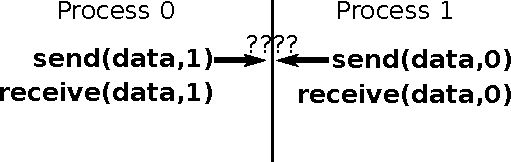
\includegraphics[scale=1]{02.MPI_pt2pt/deadlock.pdf}
\end{center}

Also non-blocking coommunication are usefull to overlap communication and computation
\end{frame}

\begin{frame}{Blocking and non-blocking communications}
\begin{green1block}{A blocking communication means\ldots}
    That the buffer can be re-used after the function as returned.
\end{green1block}
\begin{green1block}{A non-blocking communication means\ldots}
    That the buffer can only be re-used after a wait function as returned.\\
    Until then, the buffer must not be overwritten (and even read).
\end{green1block}
\begin{red1block}{\textbf{Blocking} and non-blocking do not mean\ldots}
    That the communication is completed after the function as returned.
\end{red1block}
\begin{itemize}
    \item<2>[\color{cscsred}$\Rightarrow$]\color{cscsred}\textbf{It is all about buffer availability!}
\end{itemize}
%    \includegraphics[scale=0.3]{blocksend.pdf}
%\begin{itemize}
%\end{itemize}
\end{frame}


\begin{frame}[fragile]{Blocking and non-blocking examples}
    \begin{columns}
        \begin{column}{0.45\paperwidth}
            Blocking example:
\begin{Pseudolisting}[]{}
int buf[120];
MPI_Send(buf,MPI_INT,5,...);
// after the function returns
// the communication is done
// the buffer can be re-used
but[3]=5
\end{Pseudolisting}
        \end{column}
        \begin{column}{0.45\paperwidth}
            Non-blocking example:
\begin{Pseudolisting}[]{}
int buf[120];
MPI_Isend(buf,MPI_INT,5,...);
// after the function returns
// the communication is not done
// do not overwrite buf
// buf[3]=5 illegal
MPI_Wait(...);
// here communication is done
but[3]=5
\end{Pseudolisting}
        \end{column}
    \end{columns}
Each rank does not necessary know if the communication has been completed by the time the MPI send function returns.\\
The \lstinlinePseudo{I} in \lstinlinePseudo{MPI_Isend} means {\color{cscsred}immediate}, the function returns "immediately" after its call.
\end{frame}

\begin{frame}[fragile]{Non-blocking MPI\_Isend and MPI\_Irecv}
\begin{Pseudolisting}[]{}
MPI_Isend(buf,count,type,dest,tag,comm, MPI_Request req)
MPI_Irecv(buf,count,type,source,tag,comm, MPI_Request req)
\end{Pseudolisting}
\begin{black1block}{}
\begin{tabular}{rl}
    \textbf{buf} & array of type type see table\\
    \textbf{count} & number of element of buf to be sent\\
    \textbf{type} & MPI type of buf\\
    \textbf{dest} & rank of the destination process\\
    \textbf{source} & rank of the source process\\
    \textbf{tag} & number identifying the message\\
    \textbf{comm} & communicator of the sender and receiver\\
    \textbf{req} &  identifier of the communications handle\\
\end{tabular}
\end{black1block}
\end{frame}

\begin{frame}[fragile]{Waiting for completion}
\begin{Pseudolisting}[]{}
MPI_Wait(MPI_Request req, status)
MPI_Waitall(count, MPI_Request requests[], status[])
\end{Pseudolisting}
\begin{black1block}{}
\begin{tabular}{rl}
    \textbf{req} & identifier of the communications handle\\
    \textbf{status} & array containing communication status\\
    \textbf{count} & number of element of in arrays\\
\end{tabular}
\end{black1block}
\end{frame}

\begin{frame}[fragile]{Testing for completion}
\begin{Pseudolisting}[]{}
MPI_Test(req, flag, status)
MPI_Testall(count, requests[], flag, status[])
\end{Pseudolisting}
\begin{black1block}{}
\begin{tabular}{rl}
    \textbf{req} & identifier of the communications handle\\
    \textbf{flag} & true if req has completed false otherwise\\
    \textbf{status} & array containing communication status\\
    \textbf{count} & number of element of in arrays\\
\end{tabular}
\end{black1block}
\end{frame}

\subsection{Transfer modes}
\begin{frame}{Transfer modes}
Five different communication modes are supported for the Send:
\begin{itemize}
    \item Standard Mode
    \item Synchronous Mode
    \item Buffered Mode
    \item Ready Mode
\end{itemize}
All of them can be Blocking or Non-Blocking.
\end{frame}


\begin{frame}{Transfer modes: Standard Mode}
\begin{itemize}
\item A send operation can be started whether or not a matching receive has started
\item Can be buffered or synchronous. It is up to the implementation (and not MPI standard) to decide whether outgoing messages will be buffered
\item May complete before a matching receive is posted
\item Non-local operation (in general)
\end{itemize}
\end{frame}

\begin{frame}{Transfer modes: Synchronous Mode}
\begin{itemize}
\item A send operation can be started whether or not a matching receive has started
\item The send will complete successfully only if a matching receive was posted and the receive operation has reached a certain point in its execution
\item The completion of a synchronous send not only indicates that the send buffer can be reused but also indicates that the receiver has reached a certain point in its execution (usually it has received all data)
\item Non-local operation
\end{itemize}
\end{frame}

\begin{frame}[fragile]{Transfer modes: Buffered Mode}
\begin{itemize}
\item A send operation can be started whether or not a matching receive has been posted
\item It completes whether or not a matching receive has been posted (independent from the receive)
\item The original buffer can be read and overwritten, it has been copied to user-supplied buffer
\item Buffer space is allocated on demand \lstinlinePseudo{MPI_Buffer_Attach}
\item Local operation
\end{itemize}
\end{frame}

\begin{frame}{Transfer modes: Ready Mode}
\begin{itemize}
    \item A send operation may be started only if the matching receive is already started (error otherwise)
\item The completion of the send operation does not depend on the status of a matching receive and merely indicates the send buffer can be reused
\item Used for performance reasons
\item Non-local operation
\end{itemize}
\end{frame}

\begin{frame}[fragile]{Transfer modes overview}
\small

\begin{tabular}{|l|p{3.7cm}|l|l|}
\hline
\textbf{Mode} & \textbf{Completion Condition} & \textbf{Blocking} & \textbf{Non-blocking}\\\hline
Standard send & Message sent (receive state unknown)&  \lstinlinePseudo{MPI_Send} & \lstinlinePseudo{MPI_Isend} \\\hline
Receive & Completes when a matching message has arrived & \lstinlinePseudo{MPI_Recv} & \lstinlinePseudo{MPI_Irecv} \\\hline
Synchronous send & Only completes after a matching recv() is posted and the receive operation is at some stages. & \lstinlinePseudo{MPI_Ssend} & \lstinlinePseudo{MPI_Issend} \\\hline
Buffered send & Always completes, irrespective of receiver. Guarantees the message to be buffered. & \lstinlinePseudo{MPI_Bsend} & \lstinlinePseudo{MPI_Ibsend} \\\hline

Ready send & Always completes, irrespective of whether the receive has completed. & \lstinlinePseudo{MPI_Rsend} & \lstinlinePseudo{MPI_Irsend} \\\hline
\end{tabular}


\end{frame}

\subsection{Summary}
\begin{frame}{Communication - summary}
\begin{blue2block}{Blocking send and recv}
\begin{itemize}
\item Does not mean that the process is stopped during communication.
\item It means that, at return, it is safe to use the variables involved in communication.
\end{itemize}
\end{blue2block}

\begin{blue2block}{Non Blocking send and recv}
\begin{itemize}
\item Cannot use variables involved in communication until "wait" completion functions are called.
\end{itemize}
\end{blue2block}

\begin{blue2block}{Transfer modes}
\begin{itemize}
\item Define the behaviour of the various function for point to point communication. The behaviour can be implementation dependent.
\end{itemize}
\end{blue2block}
\end{frame}

\begin{frame}[fragile]{Combined Send and Recv in one function}
\justifying
The send-receive operations combine in one call the sending of a message to one destination and the receiving of another message, from another process.
The source and destination are possibly the same.
A send-receive operation is very useful for executing a shift operation across a chain of processes.
Will block until the sending application buffer is free for reuse and until the receiving application buffer contains the received message.
\begin{Pseudolisting}[]{}
MPI_Sendrecv(sndbuf, snd_size, snd_type, rcvid, tag,
             rcvbuf, rcv_size, rcv_type, sndid, tag,
             comm, status)
\end{Pseudolisting}
\end{frame}

\begin{frame}[fragile]{Other functions}
\begin{itemize}
\item Look into incomming message before to do a recv:\\\hspace{1cm}\lstinlinePseudo{MPI_Probe, MPI_Iprobe}
\item Buffer management:\\\hspace{1cm}\lstinlinePseudo{MPI_Buffer_attach, MPI_Buffer_detach}
\item Wait functions:\\\hspace{1cm}\lstinlinePseudo{MPI_Waitany, MPI_Waitsome}
\item Test functions:\\\hspace{1cm}\lstinlinePseudo{MPI_Testany, MPI_Testsome}
\item Cancel a request:\\\hspace{1cm}\lstinlinePseudo{MPI_Cancel}
\end{itemize}
\end{frame}

\begin{frame}[fragile]{Practicals}
    \begin{brown2block}{Exercise: 02.MPI\_pt2pt}
    \begin{enumerate}
        \setcounter{enumi}{3}
    \item Parallel sum using a ring:\\
        without using \lstinlinePseudo{if (rank == 0) ... else ...}\\
        {{\small
            \begin{tabular}{|c||c|c|c|}\hline
                 & Rank 0 & Rank 1 & Rank 2\\\hline
            Send & 0 & 1 & 2 \\\hline
            Recv & 2 & 0 & 1 \\\hline\hline
            Send & 2 & 0 & 1 \\\hline
            Recv & 1 & 2 & 0 \\\hline\hline
            Send & 1 & 2 & 0 \\\hline
            Recv & 0 & 1 & 2 \\\hline
            \end{tabular}\\}}
        All ranks obtain the sum.
        \item Send and Recv neighbor ghost cells:\\
            Top to bottom for C and right to left for Fortran
        \item Identify (not solve) 4 bugs in the buffer management (only in C, no Fortran version)
    \end{enumerate}
    \end{brown2block}
\end{frame}

\section{Collective communications}
\section{Topology}
\section{Datatypes}

% THANK YOU SLIDE
\cscsthankyou{Thank you for your attention.}

\end{document}
